\documentclass[12pt]{article}
\usepackage{amsmath}
\usepackage[margin=1in]{geometry}
\usepackage{graphicx}
\graphicspath{ {images/} }
\begin{document}

\begin{center}

\textbf{George Witteman -- Homework 2}

Modeling, Simulation and Analysis\\CS 250, Spring 2018

\end{center}

\begin{enumerate}
  \item \textbf{Exercise 1}: Up The Food Chain!
  \begin{enumerate}
    \setcounter{enumii}{0}
    
  	\item
			Assumptions:
	
			\begin{itemize}
				\item The prey $Y$ always have enough food.
				\item The population of $H$ stays constant over time.
				\item $H$ hunts $Y$ and $P$ equally.
				\item The food supply of the predator $P$ is entirely dependent on $Y$.
				\item Predators $P$ never get full.
				\item The environment does not favor any particular species.
				\item The rate of change of a population is proportional to it's size.
			\end{itemize}
			
			The differential equations for this model are
			\begin{align}
				\frac{dY}{dt} &= k_{Y}Y - k_{PY}PY - fHY\\
				\frac{dP}{dt} &= -k_{P}P + k_{YP}YP - fHP\\
				\frac{dH}{dt} &= 0
			\end{align}
			where 
			\begin{itemize}
				\item $k_{Y}$ is the prey birth constant,
				\item $k_{P}$ is the predator death constant,
				\item $f$ is the fishing constant (i.e. the proportion of interactions between predators/prey and humans that lead to the death of a predator/prey),
				\item $k_{PY}$ is the proportion of interactions of predators and prey leading to the death of prey,
				\item and $k_{YP}$ is the proportion of interactions of predators and prey leading to the birth of a predator.
			\end{itemize}
			
		\item
			As the fishing rate increases, the maximum and minimum population of $P$ decrease, but the maximum and minimum population of $Y$ increase. This indicates that fishing impacts $P$ more than $Y$. This makes sense, because without $Y$ $H$ could not survive since it's $Y$ food source would be gone and it's $P$ food source would die off.
			
			Given the model, the impact of predator $H$ is most significant against the population of predator $P$, since the population of predator $P$ decreases. Increasing the fishing constant $f$ also slows the cycle of increasing/decreasing prey.
						
		\item
			The fishing rate $f$ that predators all die is when $f \ge 0.02$. In order for predators to die off they need to lose all of their food supply (i.e. $Y$). In order for this to happen $\frac{dY}{dt}$ needs to be less than or equal to 0 (i.e. $0 \ge \frac{dY}{dt} = k_{Y}Y - k_{PY}PY - fHY$). We can also ignore the term $-k_{PY}PY$ in $\frac{dY}{dt}$, since $P = 0$ when predators die off. Solving for $f$ we get $f \ge \frac{k_Y}{H}$. Since we are assuming the population of predator $H$ is constant, we can substitute the constants from my example to get $f \ge \frac{2}{100} = 0.02$.
			
		\item
			The model for this part is nearly identical to the model for Exercise 1a, except the value for the amount of fishing is dependent on time. The function to determine the values for the periodic seasonal fishing is the piecewise function
			\begin{align}
  			f(t) = 
      	\begin{cases}
					0,& t \mod 12 \le 6\\
					\frac{f_{max}}{2} + \frac{f_{max}}{2} \times \cos(\frac{2\pi}{6} \times t + \pi),& t \mod 12 > 6
      	\end{cases}
			\end{align}
			
			This function is modeled after the function given in Project 1 of Chapter 4.2 of the textbook with the values $f = \frac{f_{max}}{2}$, $a = \frac{f_{max}}{2}$, and $p = 6$ (months).
			
			One effect I noticed with this is that when the initial population for $Y$ and $P$ are close (e.g. $Y_1 = 100$ and $P_1$ = 85), then the simulation starts out relatively stable, but once the 6 month mark is reached, the population of prey starts to increase at a faster rate and the population of predators start to decrease at a faster rate. This is shortly followed by a spike in predator population and decline in prey, since there is a much larger amount of prey at this point than the predators, and the fishing amount is not large enough to prevent predators from increasing in population. See Figure \ref{fig:similarPredPrey} for an example of this.
			\begin{figure}[h]
  			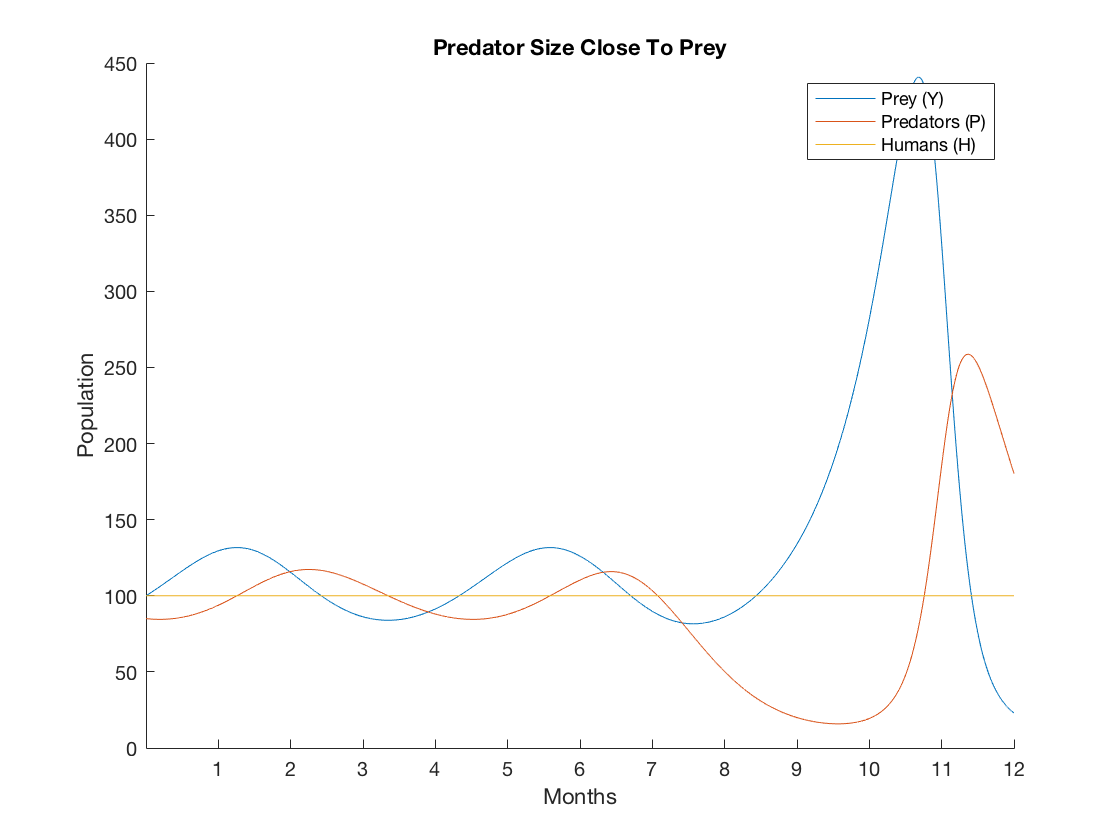
\includegraphics[width=0.75\textwidth]{1d-1}
  			\centering
        \caption{Example when the predator size is close to prey}
        \label{fig:similarPredPrey}
      \end{figure}
			
						
  \end{enumerate}
  
  \item \textbf{Exercise 2}: Change It Up!
    \begin{enumerate}
    	\item
      	Assumptions:
  		
  			\begin{itemize}
  				\item The prey $Y$ always have enough food.
  				\item $H$ hunts only $P$.
  				\item The food supply of the predator $P$ is entirely dependent on $Y$.
  				\item Predators $P$ never get full.
  				\item Humans $H$ never get full.
  				\item The environment does not favor any particular species.
  				\item The rate of change of a population is proportional to it's size.
  			\end{itemize}
  			
  			The differential equations for this model are
  			\begin{align}
  				\frac{dY}{dt} &= k_{Y}Y - k_{PY}PY\\
  				\frac{dP}{dt} &= -k_{P}P + k_{YP}YP - k_{HP}HP\\
  				\frac{dH}{dt} &= -k_{H}H + k_{PH}PH
  			\end{align}
  			where
  			\begin{itemize}
  				\item $k_{Y}$ is the prey birth constant,
  				\item $k_{P}$ is the predator death constant,
  				\item $k_{H}$ is the human death constant,
  				\item $k_{HP}$ is the proportion of interactions between predators and humans that lead to the death of a predator,
  				\item $k_{PY}$ is the proportion of interactions of predators and prey leading to the death of prey,
  				\item $k_{YP}$ is the proportion of interactions of predators and prey leading to the birth of a predator, and
  				\item $k_{PH}$ is the proportion of interactions of predators and humans leading to the birth of a human.
  			\end{itemize}
  			
  			This model is similar to the model from Exercise 1a, with a couple of differences. First, since the population of $H$ is no longer constant, $\frac{dH}{dt}$ is no longer zero. Instead, the change in population for $H$ is equal to the rate that $H$ would die off if it had no prey to eat ($-k_{H}H$) plus the number of interactions that lead to a birth of a member of $H$ ($k_{PH}PH$). I have also changed the "fishing constant" to be represented by $k_{HP}$ here instead of $f$, in order to make clearer the function that it has.
  			
  			\begin{figure}[h]
    			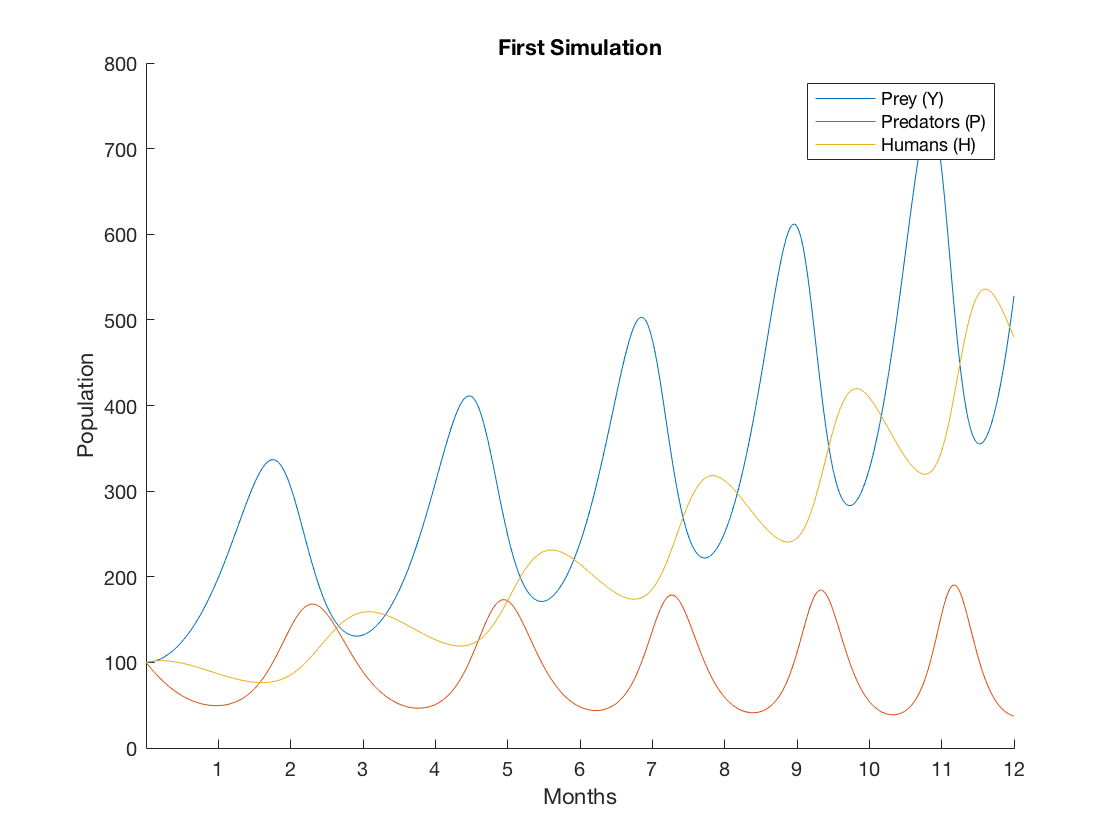
\includegraphics[width=0.75\textwidth]{2a-1}
    			\centering
          \caption{Example simulation for the model of Exercise 2a.}
          \label{fig:2a-1}
        \end{figure}
        
        To simulate this model, I used Euler's method of simulation. For each time step I calculate the number of interactions between all pairs of $Y$, $P$, and $H$ at $t-\Delta t$. Then, I calculate the change in population at $t-\Delta t$ for all populations. Finally, the population for time $t$ is calculated by adding the population at time $t-\Delta t$ to the change in population at $t-\Delta t$. In the code, $t = i * \Delta t$ for the iteration variable $i$, so $t-\Delta t = i - 1$.
        
  			An example simulation can be seen in Figure \ref{fig:2a-1}. The results of a simulation using this model where the constants are chosen such that no animal dies out are similar to the simulations of other models. There is a cyclic pattern of animal deaths, followed by a spike in the prey population since their predators population has decreased. This spike in prey population causes a spike in the population of predators, since the now have an increased access to food. The difference with this model, is that the human population now will also increase since the population of it's prey, the predator $P$, has now grown.
  			
  			Another difference between this and the previous models is that the populations of $Y$ and $H$ grow to be much larger than even the maximum population of $P$. 
  			 
  		\item
  			The assumptions of this model are the same as Exercise 2a, except that $H$ hunts both species $P$ and species $Y$ instead of just species $P$. It's also important to note that unlike the model in Exercise 1a, we do not make the assumption here that $H$ eats both $Y$ and $P$ equally. Instead $H$ may eat $Y$ or $P$ more, and thus we should have different constants for the interactions between $H$ and $Y$ and $H$ and $P$.
  			
  			 This model has the following differential equations
  			\begin{align}
  				\frac{dY}{dt} &= k_{Y}Y - k_{PY}PY - k_{HY}HY\\
  				\frac{dP}{dt} &= -k_{P}P + k_{YP}YP - k_{HP}HP\\
  				\frac{dH}{dt} &= -k_{H}H + k_{YH}YH + k_{PH}PH
  			\end{align}
  			where
  			\begin{itemize}
  				\item $k_{Y}$ is the prey birth constant,
  				\item $k_{P}$ is the predator death constant,
  				\item $k_{H}$ is the human death constant,
  				\item $k_{PY}$ is the proportion of interactions of $P$ and $Y$ leading to the death of a member of species $Y$,
  				\item $k_{HY}$ is the proportion of interactions of $H$ and $Y$ leading to the death of a member of species $Y$,
  				\item $k_{YP}$ is the proportion of interactions of $Y$ and $P$ leading to the birth of a member of species $P$,
  				\item $k_{HP}$ is the proportion of interactions of $H$ and $P$ leading to the death of a member of species $P$,
  				\item $k_{YH}$ is the proportion of interactions of $Y$ and $H$ leading to the birth of a member of species $H$, and
  				\item $k_{PH}$ is the proportion of interactions of $P$ and $H$ leading to the birth of a member of species $H$.
  			\end{itemize}
  			
  			\begin{figure}[h]
    			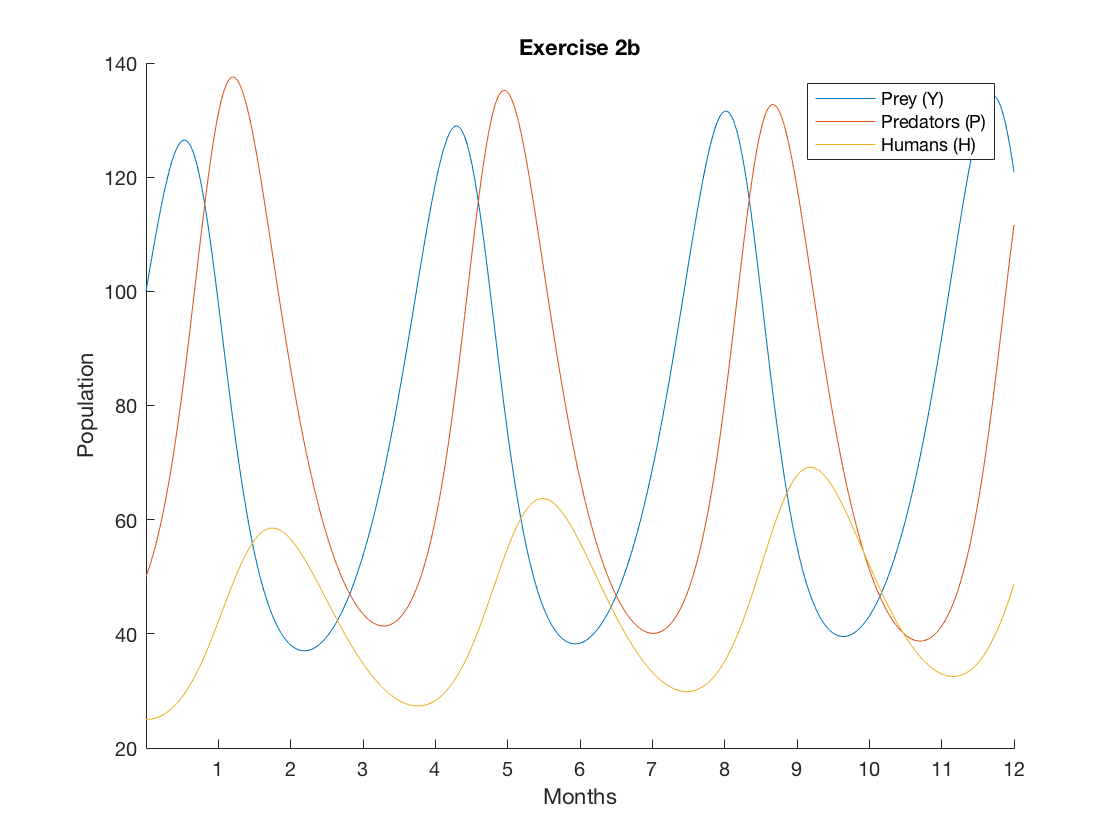
\includegraphics[width=0.75\textwidth]{2b-1}
    			\centering
          \caption{Example simulation for the model of Exercise 2b.}
          \label{fig:2b-1}
        \end{figure}
        
        Figure \ref{fig:2b-1} shows an example simulation for this model. 
        
      \item
  			One interesting question that can be asked about these models is whether it is possible for species $H$ to be the most dominant (i.e. largest population) while not depleting it's food supply of $Y$ and $P$.
			
			My primary hypothesis for this question is that it is possible for the population of $H$ to always be greater than the population of $Y$ and the population of $P$. The reasoning behind this hypothesis is that even if the population of $H$ is always greater than the population of both of it's food sources, the birth rate of the food sources could be enough such that they are always being born faster than they are getting eaten. The competing hypothesis is that it is not possible for the population of $H$ to always be greater than the population of $Y$ and the population of $P$.
			
			In order to find evidence for/against this hypothesis, I ran the simulation with multiple sets of values for the constants. I was able to find at least one example where $H$ is always greater than the populations of it's prey. The parameters that I used are $k_{Y} = 2$, $k_{P} = 1$, $k_{H} = 1.5$, $k_{PY} = 0.01$, $k_{YP} = 0.01$, $k_{HP} = 0.01$, $k_{YH} = 0.03$, $k_{PH} = 0.03$, and $Y_{1} = P_{1} = H_{1} = 50$. The plot generated by these parameters is in Figure \ref{fig:2c-1}.
			
			\begin{figure}[h]
  			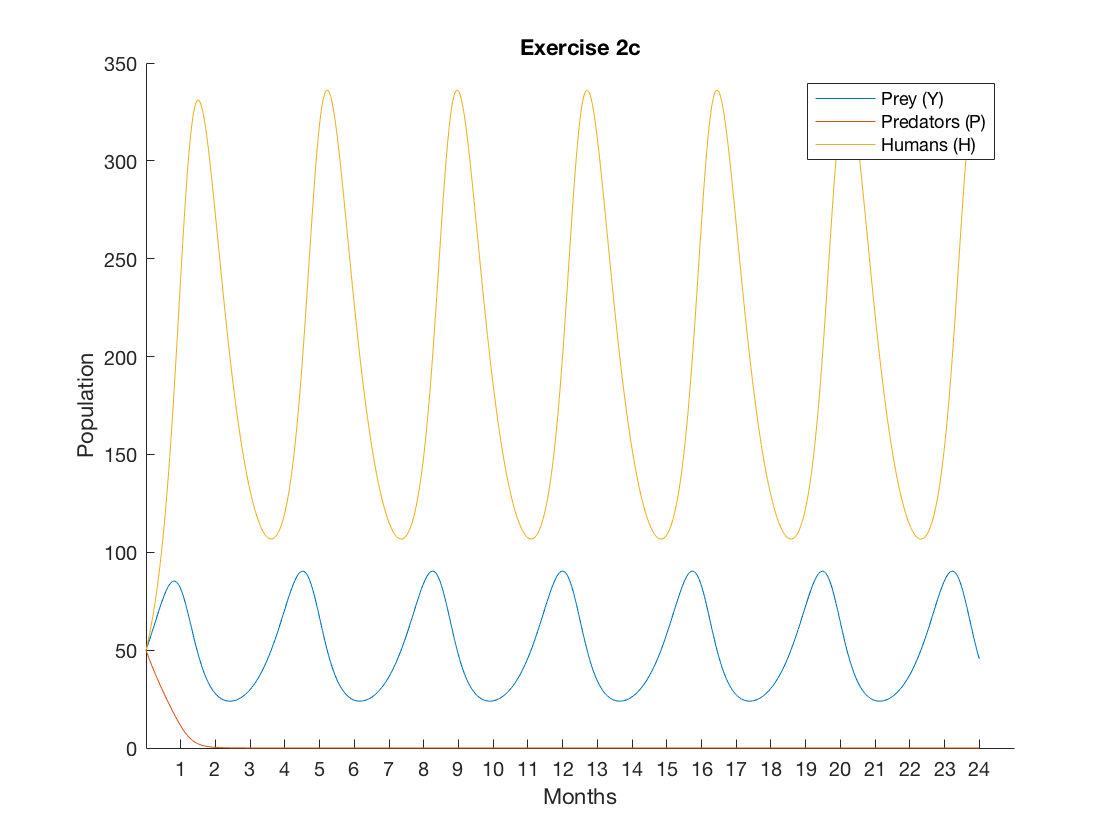
\includegraphics[width=0.75\textwidth]{2c-1}
  			\centering
        \caption{One example simulation that proves the primary hypothesis for Exercise 2c.}
        \label{fig:2c-1}
      \end{figure}
      
      Figure \ref{fig:2c-1} shows that it is possible for $H$ to always be greater than $Y$ and $P$, however in this case we see that $P = 0$. The population of $P$ is quickly drawn down to 0 by both the rapid increase in the population of $H$ and also the decrease in the size of population $Y$.
      
      I arrived at this set of constants using a number of different strategies to choose constants. First, it's important that $Y$ does not die out, because both $P$ and $H$ are reliant on $Y$ for food either directly, as in $P$, or indirectly, as in $H$. Therefore, $k_{Y}$ needs to be a relatively large number in order to have enough $Y$ being born. Second, $k_{H}$ needs to be small enough so that $H$ is not decreasing too quickly at any given point, but also large enough that $H$ is not eating all the other species. Third, $k_{YH}$ and $k_{PH}$ need to be sufficiently high so that $H$ is growing quick enough to stay above $Y$ and $P$.
      
      By trying out different combinations of constants that worked with these parameters, I was able to find a set of constants that worked to give an example case that shows the primary hypothesis.
  		
  	\end{enumerate}  
  
  \end{enumerate}

\end{document}